\documentclass{article}
\thispagestyle{empty}
\usepackage{amsmath}
\usepackage{tikz}
\usepackage{tikz-cd}
\usetikzlibrary{%
  matrix,%
  calc,%
  arrows%
}

\DeclareMathOperator{\coker}{coker}

\begin{document}
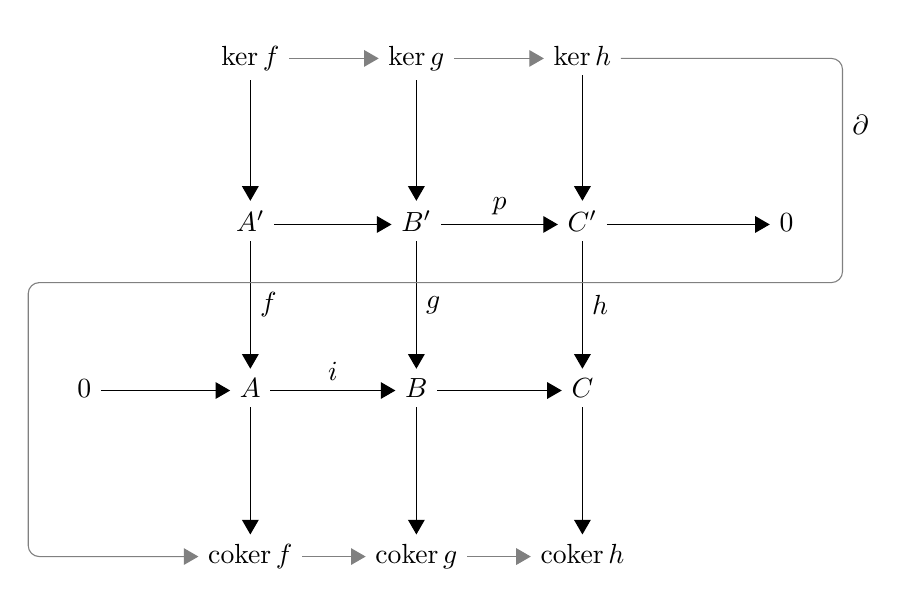
\begin{tikzpicture}[>=triangle 60]
\matrix[matrix of math nodes,column sep={60pt,between origins},row
sep={60pt,between origins},nodes={asymmetrical rectangle}] (s)
{
&|[name=ka]| \ker f &|[name=kb]| \ker g &|[name=kc]| \ker h \\
%
&|[name=A]| A' &|[name=B]| B' &|[name=C]| C' &|[name=01]| 0 \\
%
|[name=02]| 0 &|[name=A']| A &|[name=B']| B &|[name=C']| C \\
%
&|[name=ca]| \coker f &|[name=cb]| \coker g &|[name=cc]| \coker h \\
};
\draw[->] (ka) edge (A)
          (kb) edge (B)
          (kc) edge (C)
          (A) edge (B)
          (B) edge node[auto] {\(p\)} (C)
          (C) edge (01)
          (A) edge node[auto] {\(f\)} (A')
          (B) edge node[auto] {\(g\)} (B')
          (C) edge node[auto] {\(h\)} (C')
          (02) edge (A')
          (A') edge node[auto] {\(i\)} (B')
          (B') edge (C')
          (A') edge (ca)
          (B') edge (cb)
          (C') edge (cc)
;
\draw[->,gray] (ka) edge (kb)
               (kb) edge (kc)
               (ca) edge (cb)
               (cb) edge (cc)
;
\draw[->,gray,rounded corners] (kc) -| node[auto,text=black,pos=.7]
{\(\partial\)} ($(01.east)+(.5,0)$) |- ($(B)!.35!(B')$) -|
($(02.west)+(-.5,0)$) |- (ca);
\end{tikzpicture}
\end{document}